\fontfamily{\sfdefault}\selectfont
% XCircuit output "bbpll.tex" for LaTeX input from bbpll.ps
\def\putbox#1#2#3#4{\makebox[0.00000in][l]{\makebox[#1][l]{}\raisebox{\baselineskip}[0.00000in][0.00000in]{\raisebox{#2}[0.00000in][0.00000in]{\scalebox{#3}{#4}}}}}
\def\rightbox#1{\makebox[0.00000in][r]{#1}}
\def\centbox#1{\makebox[0.00000in]{#1}}
\def\topbox#1{\raisebox{-0.60\baselineskip}[0.00000in][0.00000in]{#1}}
\def\midbox#1{\raisebox{-0.20\baselineskip}[0.00000in][0.00000in]{#1}}
   \scalebox{1}{
   \normalsize
   \parbox{3.10000in}{
   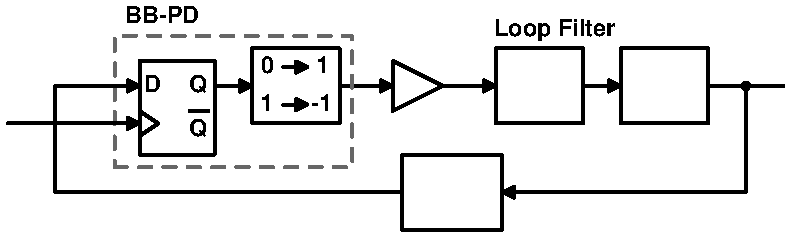
\includegraphics[scale=0.60000]{./figs/bbpll.pdf}\\
   % translate x=1336 y=392 scale 0.38
   \putbox{1.63200in}{0.70800in}{0.72}{$K_{bb}$}%
   \putbox{1.69800in}{0.14400in}{0.72}{$\div$ N}%
   \putbox{2.55600in}{0.57000in}{0.72}{DCO}%
   \putbox{2.01000in}{0.57000in}{0.72}{H$_{LF}$(z)}%
   \putbox{0.06000in}{0.51000in}{0.72}{Clk}%
   \putbox{2.89800in}{0.66000in}{0.72}{Out}%
   } % close 'parbox'
   } % close 'scalebox'
   \vspace{-\baselineskip} % this is not necessary, but looks better
\fontfamily{\rmdefault}\selectfont
